
\chapter{Spectrogram}

The spectrogram is the most common tools used in order to do a time frequency representation. This representation use the short-time-Fourier transformation in order to apply an fast-Fourier transformation on a slippery window of the signal. In the end, we get an image which represent the frequency which compose the signal at an instant t given.

Let consider the signal chirp below which correspond to a signal which its frequency increases from 0 to 300Hz.

\begin{figure}[H]
\centering
    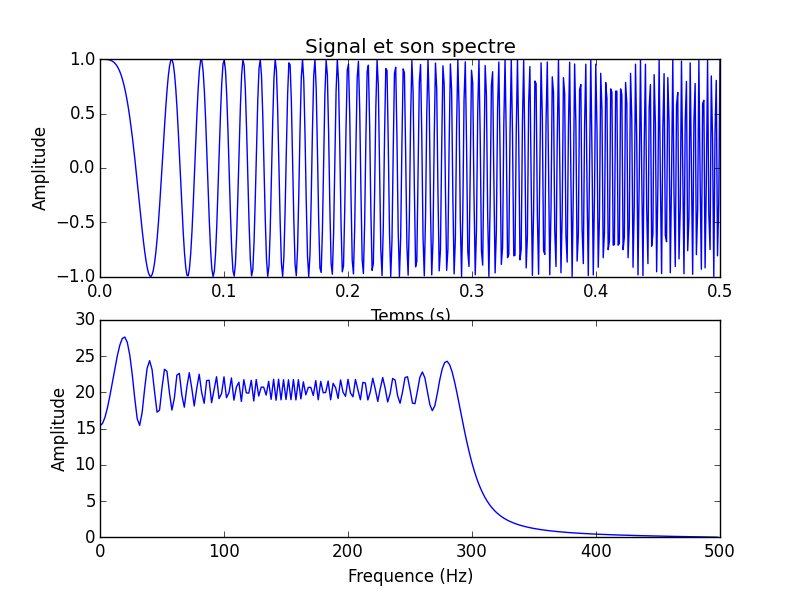
\includegraphics[scale=0.6,angle=0]{ChirpTF.png}
    \caption{Time and frequency representation of a chirp signal.}
    \label{fig:ChirpTF}
\end{figure}

The figure below shows the results we can get:

\begin{figure}[H]
\centering
    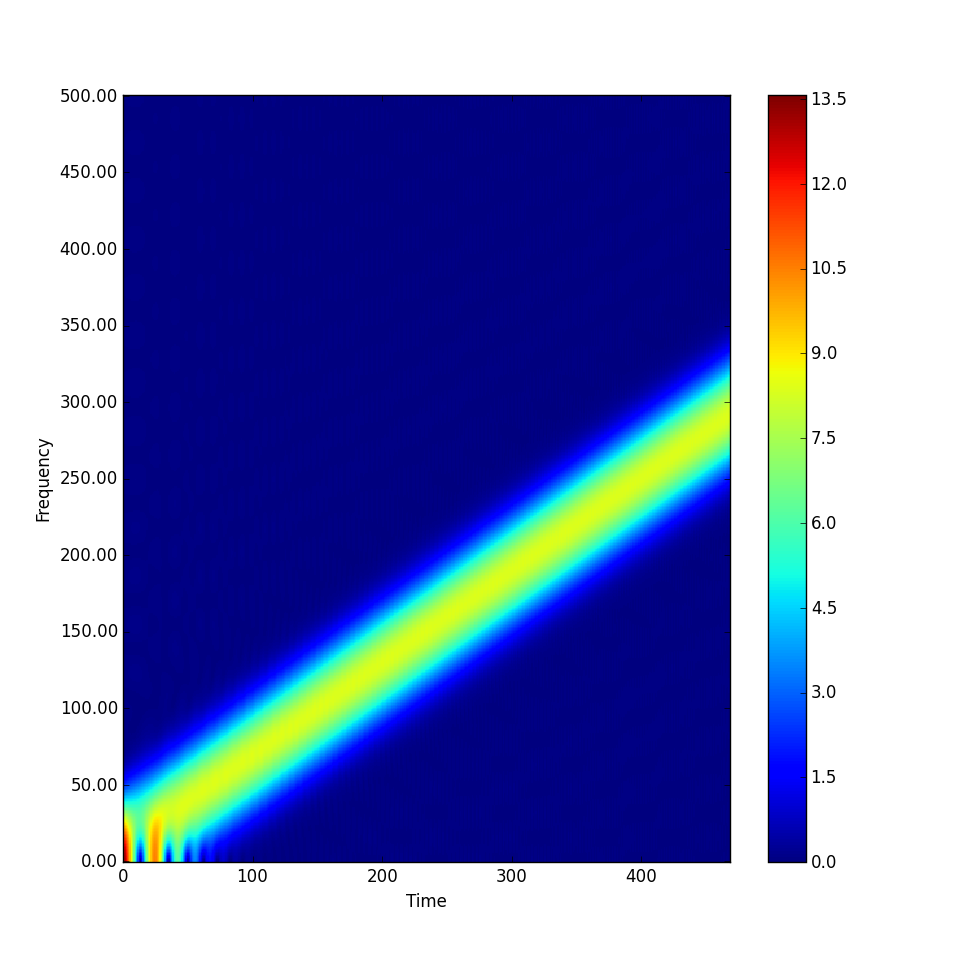
\includegraphics[scale=0.6,angle=0]{Chirp_STFT.png}
    \caption{STFT/spectrogram of a chirp signal.}
    \label{fig:Chirp_STFT}
\end{figure}

This figure shows clearly that the frequency of the signal increass through time but the result is a little blur and isn't very accurate.

\chapter{Wigner-Ville}

The Wigner-Ville distribution allows us to get a far more accurate time frequency representation. Nevertheless, this distribution create some interferences if the signal is a combination of different frequency laws.

The Wigner-Ville Distribution (WVD) of a signal y(t), denoted by $W_z(t,f)$, is defined as :

\begin{equation}
W_z(t,f) = \int_{n=-\infty}^{\infty} z ( t + \tau / 2 ) z^* (t - \tau / 2) e^{-j 2 \pi f \tau d \tau}
\end{equation}

The following figure shows the result of the Wigner-Ville representation on the previous signal:

\begin{figure}[H]
\centering
    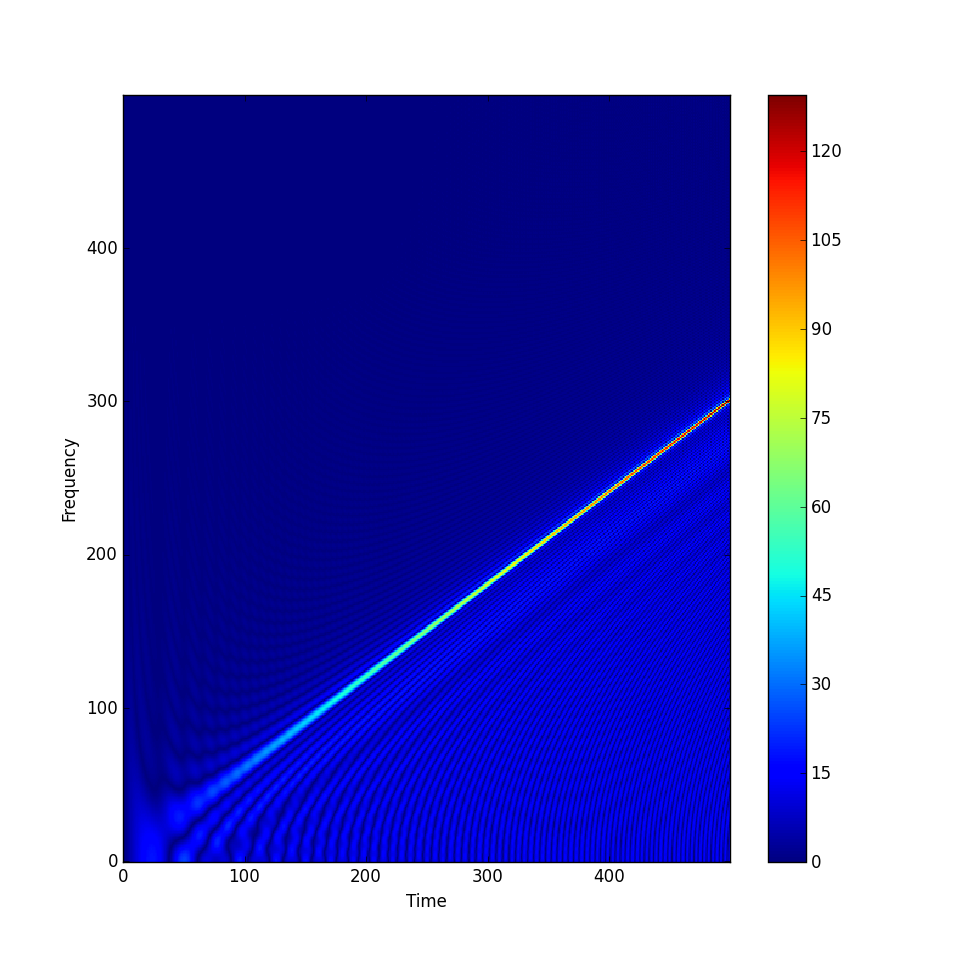
\includegraphics[scale=0.5,angle=0]{Chirp_WV.png}
    \caption{Wigner-Ville of a chirp signal.}
    \label{fig:Chirp_WV}
\end{figure}

Nevertheless, if we consider the following signal which contains two sinusoids, with different frequency and with one which last for only a portion of the signal. We get the result below:

\begin{figure}[H]
\centering
    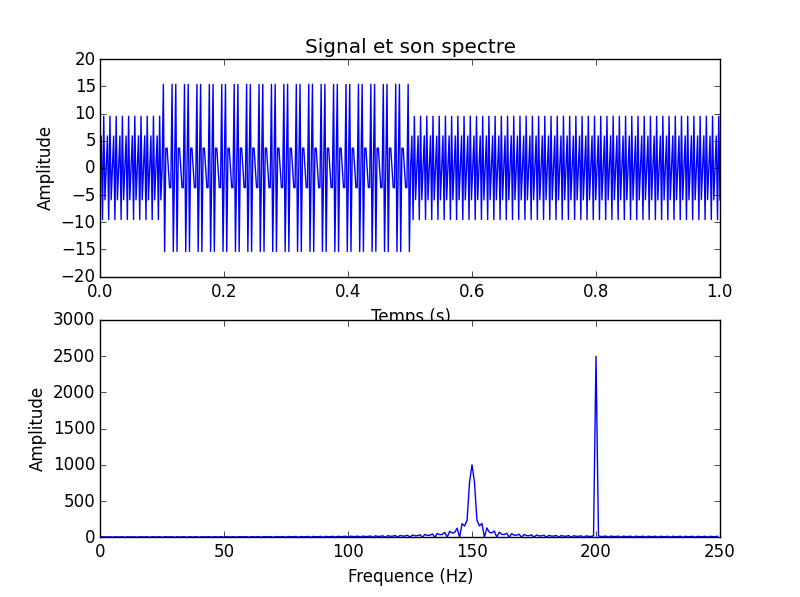
\includegraphics[scale=0.5,angle=0]{SignalSimple.png}
    \caption{Time and frequency representation of the signal with two frequency laws.}
    \label{fig:SignalSimple}
\end{figure}

\begin{figure}[H]
\centering
    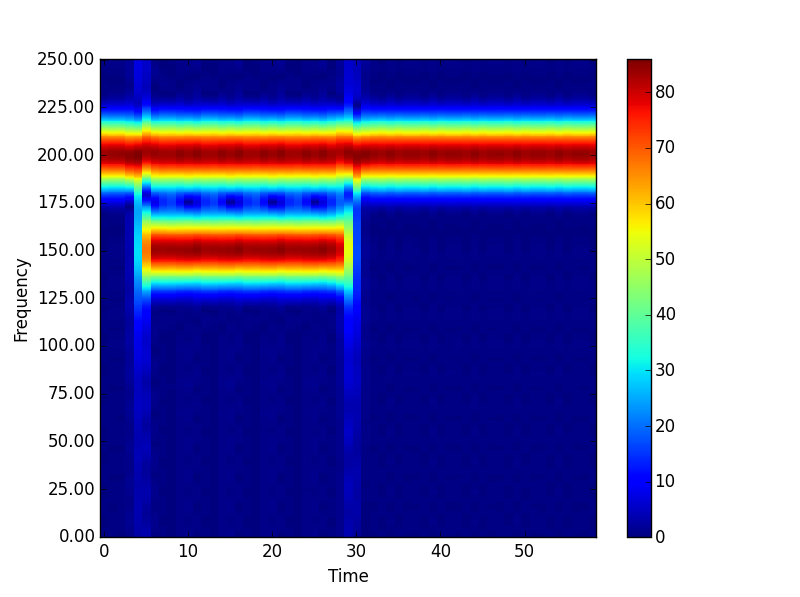
\includegraphics[scale=0.5,angle=0]{figure_6STFT.png}
    \caption{Spectrogram of the signal.}
    \label{fig:SignalSimple_Spectrogram}
\end{figure}

\begin{figure}[H]
\centering
    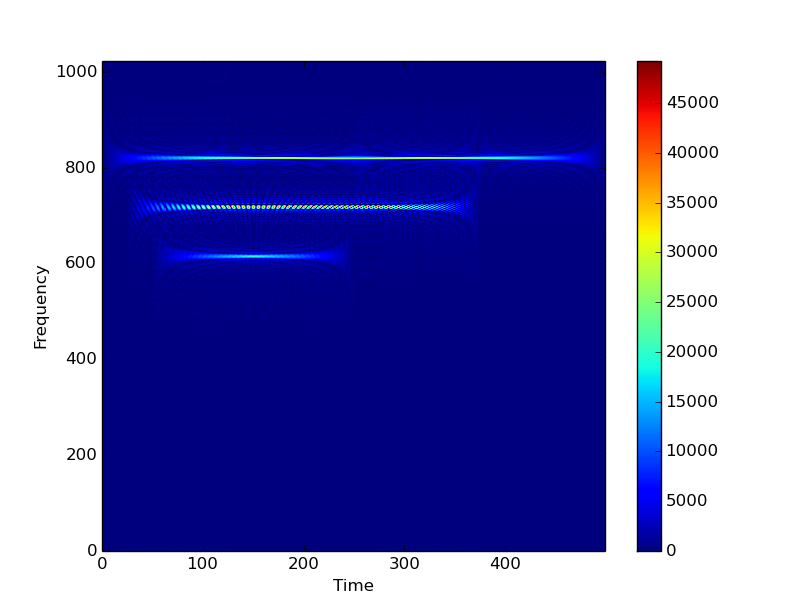
\includegraphics[scale=0.5,angle=0]{SignalSimple_WV.png}
    \caption{Wigner-Ville of the signal.}
    \label{fig:SignalSimple_WV}
\end{figure}

As you can see, there are an interference which imply to analyse this figure if we want to extract relevant information.

\textbf{NB :} The differences in the frequency scale is due to a problem in the implementation I realized. I will correct this as soon as I can.

\chapter{Pseudo Smooth Wigner-Ville}

The  Pseudo-Wigner-Ville Distribution is defined as:

\begin{equation}
W_z(t,f) = \int_{n=-\infty}^{\infty} h ( \tau ) z ( t + \tau / 2 ) z^* (t - \tau / 2) e^{-j 2 \pi f \tau d \tau}
\end{equation}

where $h$ is a regular window. This windowing is equivalent to a frequency smoothing of the WVD so It leads to the attenuation of the interference terms but it will damage the signal representation.

The result for the previous signal is below:

\begin{figure}[H]
\centering
    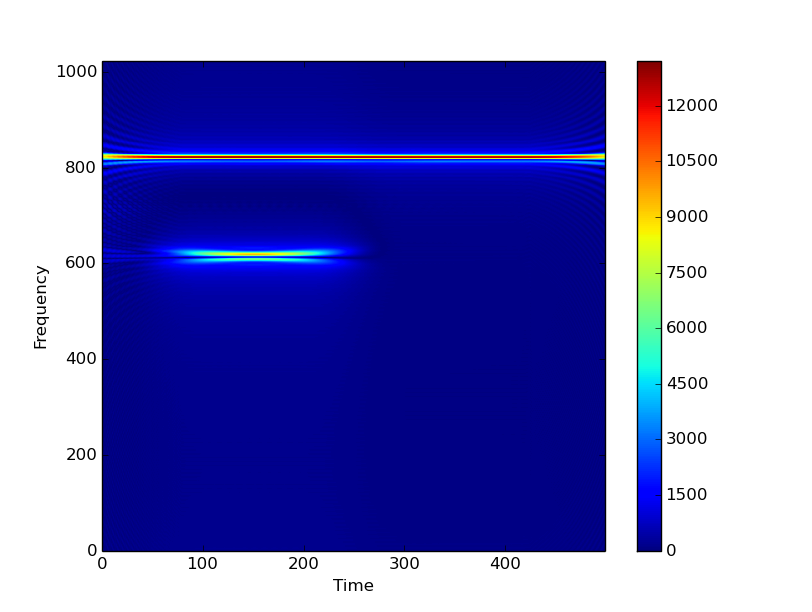
\includegraphics[scale=0.5,angle=0]{SignalSimple_PSWV.png}
    \caption{Pseudo Smooth Wigner-Ville of the signal.}
    \label{fig:SignalSimple_PSWV}
\end{figure}

\chapter*{Conclusion}
\bigskip
All those representation present some interests or disadvantages. Nevertheless, if we want to get as much information as we can, we will need to switch between a representation to another according to the kind of signal we have. At the beginning of the project, an implementation of the Flandrin library coming from Matlab was implemented but we found afterwards a python library which was already doing this part. The following link shows the function of this library and the second one explain how it can be install on your computer. The previous pictures came from our own functions but the next pictures will use the function of this library.

\medskip

\textit{https://github.com/scikit-signal/pytftb}

\medskip

\textit{http://pytftb.readthedocs.org/en/master/}

\medskip

All the time frequency representation of this project now use those function which provide a much more reliable result than the function we tried to implemented.
